% 使用 xelatex 编译
\documentclass[UTF8,a4paper,twoside,zihao=-4]{ctexrep}
%%%% 文档类设置 %%%%%%%%
\ctexset{
	contentsname = {目\quad 录},
	chapter = {
		beforeskip = 0pt,
		afterskip = 20pt,
		name = {第,章},
		nameformat = \zihao{3}\bfseries,
		number = \Chinese{chapter},
		numberformat = \zihao{3}\bfseries,
		titleformat = \zihao{3}\bfseries,
		fixskip = true,
		%afterindent = false
		        },
	section = {
		beforeskip = \ccwd,
		afterskip =1ex plus 0.2ex,
		format = \raggedright,
		nameformat = \zihao{4}\bfseries,
		numberformat = \zihao{4}\bfseries,
		titleformat = \zihao{4}\bfseries,
		%afterindent = false
			},
	subsection = {
		beforeskip =\ccwd,
		afterskip = 0.5ex,
		format = \raggedright,
		nameformat = \zihao{-4}\bfseries,
		numberformat = \zihao{-4}\bfseries,
		titleformat = \zihao{-4}\bfseries
			}
	    }

%%%% 宏包 %%%%%%%%%%%
\usepackage{amsmath,amssymb,amsfonts,mathrsfs}
\usepackage{graphicx}
\usepackage{tikz}
\usepackage{ulem}
\usepackage{pdfpages}
\usepackage{lipsum}
\usepackage{booktabs}
\usepackage{enumerate }
\usepackage[colorlinks,linkcolor=blue,citecolor=blue,bookmarks=true,bookmarksnumbered=true]{hyperref}
\usepackage[round]{natbib}
%%%%% 定理环境 %%%%%%%%%
\usepackage[thmmarks]{ntheorem}
{
  \theoremstyle{nonumberplain}
  \theoremheaderfont{\indent\bfseries}
  \theorembodyfont{\normalfont}
  \theoremsymbol{\ensuremath{\Box}}
  \newtheorem{proof}{证明}
}
{
  \theoremheaderfont{\indent\bfseries}
  \theorembodyfont{\normalfont}
  \newtheorem{theorem}{定理}[chapter]
  \newtheorem{lemma}{引理}[chapter]
  \newtheorem{definition}{定义}[chapter]
}
%%%%%% 图表标题设置 %%%%%%%%%%%%%%%
\usepackage{caption}
\DeclareCaptionLabelFormat{mylabel}{{\xeCJKsetup{CJKecglue={\hskip 0pt}}#1#2}}
\captionsetup{
		font= small,
		labelfont = bf,
		labelsep = space,
		labelformat = mylabel
			}
\makeatletter
\renewcommand{\thefigure}{\ifnum \c@chapter>\z@ \thechapter-\fi \@arabic\c@figure}
\renewcommand{\thetable}{\ifnum \c@chapter>\z@ \thechapter-\fi \@arabic\c@table}
\makeatother

%%%% 页面设置 %%%%%%%%%%%%%%%%%%%%%%
\usepackage[bindingoffset=.5cm,centering,includeheadfoot,margin=2.5cm,headsep=1em]{geometry}
\setlength\parskip{0pt}
\usepackage{fancyhdr}\pagestyle{fancy}
\renewcommand\chaptermark[1]{%
	\markboth{\CTEXthechapter\quad #1}{}}
\renewcommand\sectionmark[1]{%
	\markright{\CTEXthesection\quad #1}}
\fancyhf{}
\fancyhead[LE,RO]{\thepage}
\fancyhead[RE]{\textsl{\nouppercase{\leftmark}}}
\fancyhead[LO]{\textsl{\nouppercase{\rightmark}}}
%\renewcommand{\headrulewidth}{0pt}
	
	
%%%% 字体 %%%%%%%%%
% xelatex 默认字体为Latin Modern
%%%%% 自定义命令 %%%%%%%%%%%%
\newcommand{\nn}{\mathbf{N}^\ast}
\renewcommand{\leq}{\leqslant}
\renewcommand{\geq}{\geqslant}
\renewcommand{\ref}{\autoref}
\renewcommand{\epsilon}{\varepsilon}
%%%%%%%%%%%%%%%%%%%%%%
%%%%%%%%%%%%%%%%%%%%%%
\begin{document}
\bibliographystyle{plainnat}
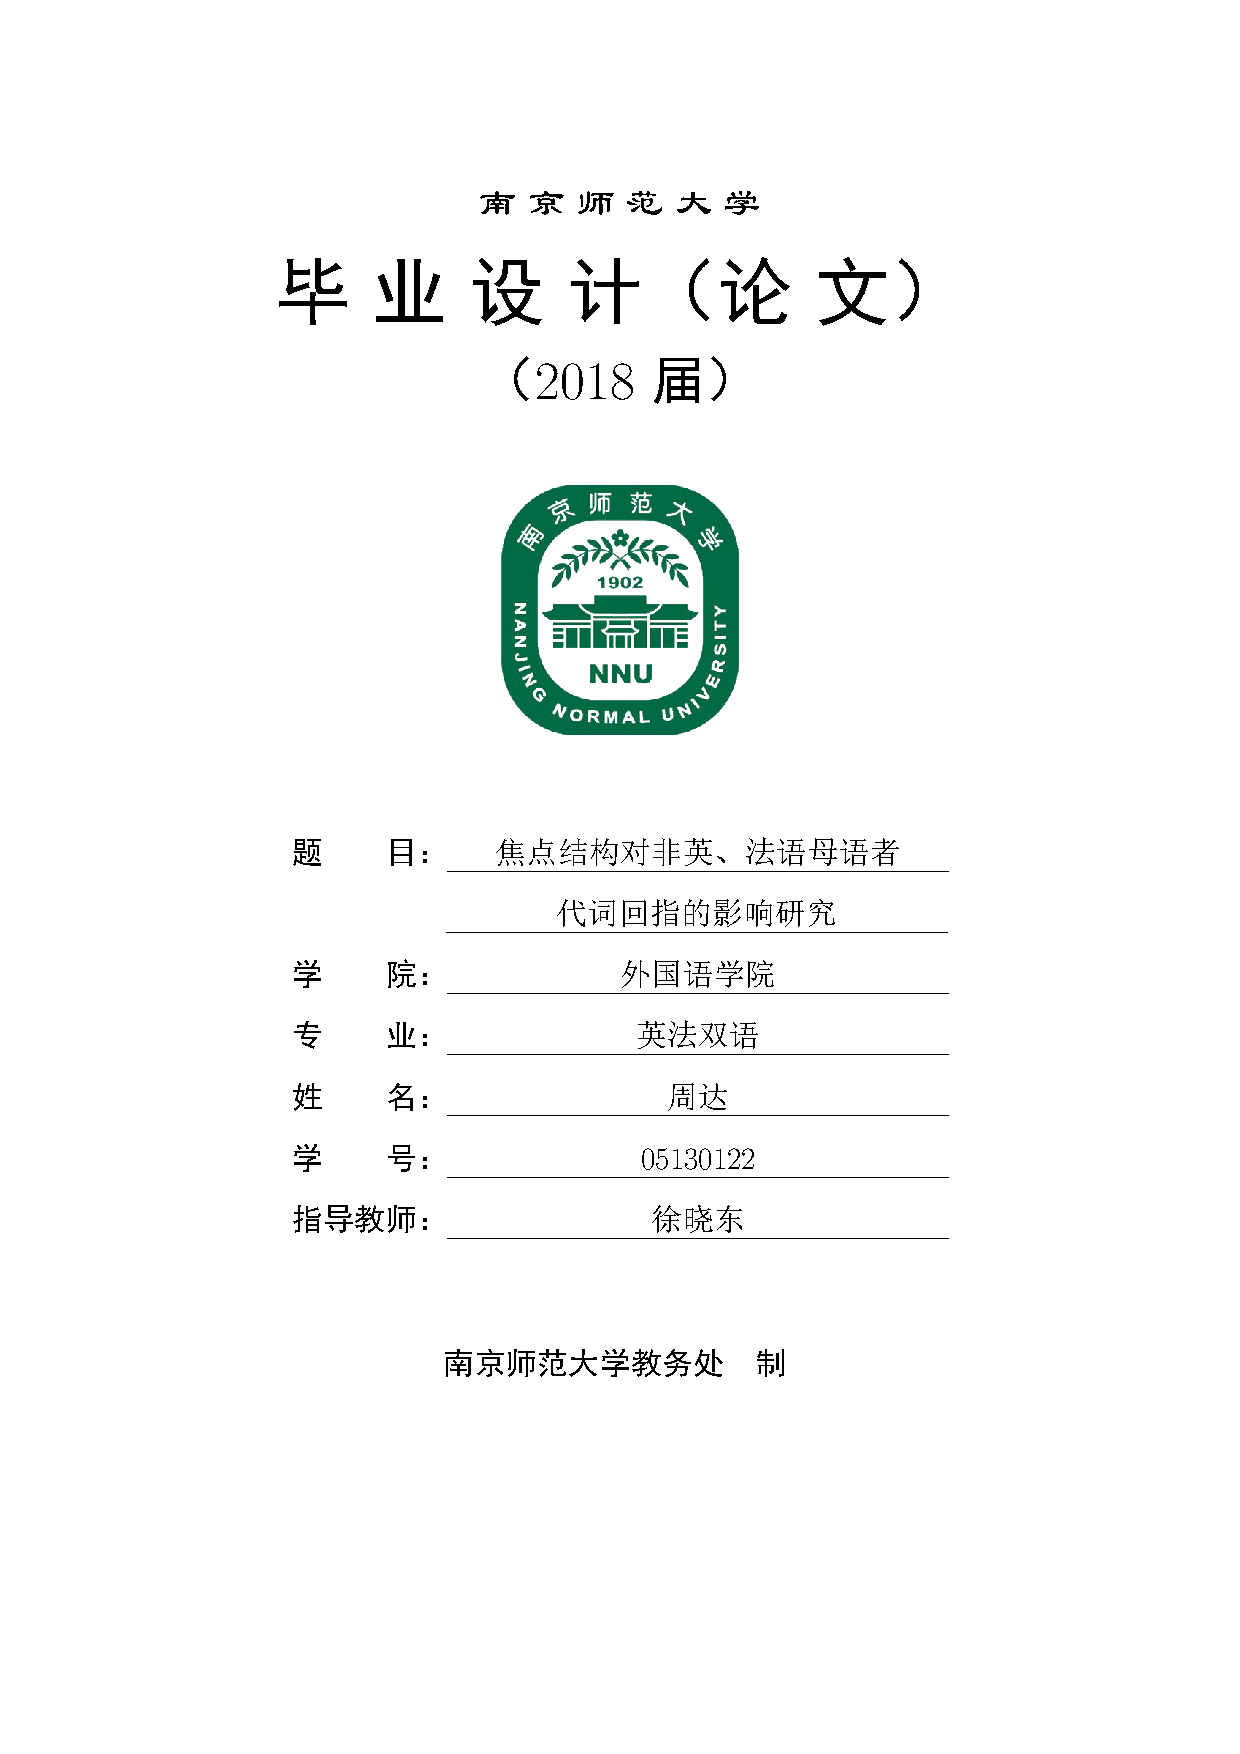
\includepdf{cover/cover.pdf} %%%%% 封面 %%%%%%%%%%%%
%%%%%%% 中英文摘要 %%%%%%%%%%%%%%%%
\pagenumbering{roman}
%%% 中文摘要
\clearpage
\thispagestyle{plain}
\phantomsection
\addcontentsline{toc}{chapter}{摘\quad 要}

\centerline{\zihao{3}\heiti 摘\quad 要}

\linespread{1.4}\zihao{-4} \bigskip

本文探讨了英语和法语非母语者的语言处理过程中,焦点结构和代词回指之间的关系。首先我们从语法和语用角度,梳理了关于焦点作用和代词回指机制的研究现状。接着通过设计自定步速阅读实验,我们发现以分裂句为形式的焦点结构不一定能提升语言片段的显著性,并使其更可能成为代词回指的对象,这与前人的研究结果是相符的。在我们的测试中,法语主语位置的焦点和英语宾语位置的焦点反应时间都较短,但两种语言的主语焦点都导致了更长的回指反应时间。另外,我们还发现焦点和回指对象的一致性并不能提升焦点位置的显著性。因此本文认为,英语和法语中是否存在主语或宾语回指偏向的问题,比当前已有研究结论更加复杂。
\bigskip

\noindent{\zihao{4}\heiti 关键词:}
焦点作用, 代词回指, 自定步速阅读, 英语, 法语

% Abstract
\clearpage
\thispagestyle{plain}
\phantomsection
\addcontentsline{toc}{chapter}{Abstract}

\centerline{\zihao{3}\bfseries Abstract}

\linespread{1.4}\zihao{-4}
\bigskip

This thesis explores the relationship between focus structure and pronoun resolution among non-native speakers of English and French. Firstly we reviewed the existing literature on the mechanism of focus effect and pronoun resolution. Then through a self-paced reading test, we find that focus, in the form of cleft structure does not necessarily increase the salience of a informational unit, thus may not in some cases make it a preferred antecedent for pronoun resolution. This result is line with previous researches on this topic. In our experiment, We also find that focused subject in French and focused object in English are processed faster, but focused subjects in both languages leads to longer response time of anaphora. Furthermore, our research also shows that the congruence between anaphora and focus does not make the latter more accessible. In this regard, we argue that the problem of whether there is subject or object preference in English and French is more complicated than the results of current studies.

\bigskip
\noindent\textbf{\zihao{4} Keywords:} 
focus effect, pronoun resolution, self-paced reading, English, French


\tableofcontents\newpage\mbox{}\thispagestyle{empty}\newpage
\clearpage\pagenumbering{arabic}
\chapter{绪论}
南京师范大学坐落在六朝古都南京,是国家“211工程”重点建设的江苏省属重点大学。它的主源可追溯到1902年创办的三江师范学堂,该学堂是中国高等师范教育的发祥地之一。后历经两江优级师范学堂、南京高等师范学校、东南大学、第四中山大学、江苏大学、中央大学、南京大学等时期;其另一源头为1888年创办的汇文书院,后发展为私立金陵大学,1951年与私立金陵女子文理学院(曾称私立金陵女子大学)合并,成立公立金陵大学。1952年全国高校院系调整,在原南京大学、金陵大学等有关院系的基础上组建南京师范学院,校址设在原金陵女子大学校址。1984年改办成南京师范大学。1996年进入国家``211工程''高校行列。2000年南京动力高等专科学校并入。目前,学校正着力建设“综合性强,办学特色鲜明,国内一流的教学研究型大学”,并为今后建成“有国际影响的高水平大学”奠定坚实基础。
\begin{figure}[htb]
    \centering
    
\includegraphics[scale=.6]{cover/nnu_caligraphy.png}
    \caption{南师大校名书法}\label{fig:caligraphy}
\end{figure}

南京师范大学作为一所百年老校,名家大师辈出,文化底蕴深厚。李瑞清、江谦、郭秉文、李叔同、张士一、陶行知、陈鹤琴、吴贻芳、孟宪承、徐悲鸿、高觉敷、潘玉良、张大千、唐圭璋、傅抱石、陈邦杰、陈洪、吴作人、李旭旦、孙望等诸多蜚声海内外的专家学者曾在此主政或执教。目前更有一大批国内外知名的专家学者在此潜心耕耘,著书立说,培育后学。经过一代又一代南师人薪火相继、身教言传,历史性地生成了``严谨朴实''的学术品格,育就了“以人为本”的厚生传统,砥砺出``团结奋进''的拼搏意识,塑造了``追求卓越''的创新精神。学校以``正德厚生、笃学敏行''为校训,形成了``严谨、朴实、奋发、奉献''的优良校风。
   
\section{南京师范大学简介} 
南京师范大学拥有仙林、随园、紫金三个校区,随园校区有着“东方最美丽的校园”之美誉。学校占地面积2009906平方米,建筑总面积1053697平方米。设有二级学院26个、独立学院2个。共有在职教职工3213人,专任教师1898人,其中正高级职称555人,副高级职称680人;中国科学院院士1名,国家级有突出贡献专家9名,``百千万人才工程''国家级人选9名,教育部创新团队1个、长江学者特聘教授5名,国家``千人计划''人才3名,国家``千人计划''青年人才2名,国家杰出青年科学基金获得者8名,国家级教学团队4个、国家教学名师3人,国家 “万人计划”人选6人,教育部``新世纪优秀人才支持计划''人选13人,中科院``百人计划''人选3人。共有在校普通本科生16763人,其中师范生3951人。在校研究生共10830人(学术型6212人,专业型4618人),其中博士研究生1246人,硕士研究生9584人。成人高等学历教育在籍生5216人。图书馆为全国古籍重点保护单位,总建筑面积44605平方米,馆藏纸本文献总量349.24万册,电子数据库106个。校园里拥有2 个“全国重点文物保护单位”。
\begin{figure}[htb]
    \centering
    
\includegraphics[scale=.4]{cover/Nanjing_Normal_University_logo.png}
    \caption{南师大校徽}\label{fig:logo}
\end{figure}

南京师范大学充分发挥``211工程''建设的主导作用和学科学位点建设的龙头作用。目前拥有国家重点学科6个、国家重点(培育)学科3个,江苏高校优势学科10个,江苏省一级学科国家重点学科培育建设点5个,江苏省一级学科重点学科23个。2011年成立研究生院。拥有博士学位授权一级学科23个、博士学位授权二级学科专业(不含一级学科覆盖)3个,硕士学位授权一级学科37个、硕士学位授权二级学科专业(不含一级学科覆盖)10个,博士专业学位类别1个,硕士专业学位类别18个,本科招生专业(含专业类)77个,博士后科研流动站22个。学科已涉及哲、经、法、教、文、史、理、工、农、医、管、艺等门类。7个学科在全国第三轮学科评估中进入全国前十,5个学科跻身ESI全球前1\%\footnote{一个脚注}。

南京师范大学不断推进``厚生育才''战略,深化教育教学改革,提高人才培养质量。拥有国家精品课程13门、国家级精品视频公开课8门、国家级精品资源共享课15门、教育部双语教学示范课程7门、教育部来华留学英语授课品牌课程2门、全国高校职业发展与就业指导示范课程1门,教育部“马工程”重点教材相应课程“精彩一课”11门,国家特色专业8个,``十二五''本科国家级规划教材21本(部),国家级教学成果奖17项,国家级人才培养模式创新实验区3个,教育部专业综合改革试点项目1个,教育部卓越教师培养计划改革项目2个,国家实验教学示范中心2个、国家文科基础学科人才培养和科学研究基地、国家理科基础学科研究和教学人才培养基地、国家体育与艺术师资培养培训基地、教育部高校辅导员培训和研修基地、大学生文化素质教育基地、国家级虚拟仿真实验教学中心、国家大学生校外实践教育基地、国家卓越法律人才教育培养基地各1个。本科教学工作水平被教育部评为优秀,被列为江苏省内本科自主招生试点单位;学生在“挑战杯”等全国竞赛中多次获得特等奖或一等奖,4篇论文入选全国优秀博士学位论文。

南京师范大学积极实施``顶天立地''战略,科研成果追求原创,力攀高峰。拥有国家地方联合工程研究中心、教育部人文社会科学重点研究基地、教育部重点实验室、公安部重点实验室、国家体育总局体育社会科学研究基地和体育文化研究基地、全国妇联妇女与性别研究与培训基地、江苏省国家重点实验室培育建设点各1个。近些年来,获得国家社会科学基金重大项目15项、教育部哲学社会科学研究重大课题攻关项目4项、国家科技支撑计划项目2项、国家重大科学研究计划项目4项、863计划主题项目课题1项、国家自然科学基金重点项目14项;在国际权威学术期刊《科学》和《自然》上发表第一作者单位论文6篇,获国家自然科学奖二等奖1项(第一单位),教育部高等学校科学研究优秀成果奖人文社会科学一等奖6项、自然科学一等奖3项(第一单位),10部专著入选“国家社科基金优秀成果文库”,科研成果入选2008年度“中国高等学校十大科技进展”和“中国基础研究十大新闻”。我校教师主持、历时8年修订的点校本《史记》,入选《光明日报》“2013十大文化亮点”和《中华读书报》“2013十大文化事件”。

\subsection{研究与合作}
南京师范大学坚持协同创新,主动为经济建设和社会发展作贡献。拥有江苏高校协同创新中心4个,江苏省哲学社会科学重点研究基地3个,江苏新型高端智库1个,江苏省决策咨询研究基地3个,江苏省委宣传部省级重点研究基地2个,江苏高校哲学社会科学重点研究基地6个(含培育点1个)、江苏省非物质文化遗产研究基地1个、江苏省学生体质健康促进研究中心1个、江苏省老年学研究基地1个;江苏省国家重点实验室建设培育点1个、江苏省重点实验室11个、工程研究中心6个,江苏省工程实验室6个,江苏省渔业重点实验室2个,江苏省科技公共技术服务平台2个。依托优势学科和重点研究机构,并通过在地方建设一批卓有成效的产学研合作平台,促进了科技成果转化和文化创意产业发展,形成了一批富有自身特色的产学研合作领域。鼓励教师开展应用对策研究,积极发挥“智囊团”和“思想库”作用。
\begin{table}[htb]\caption{某校学生身高体重样本}\label{tb:hw}
\centering\zihao{5}
\begin{tabular}{ccccc}
	\toprule
	序号 & 性别 & 年龄 & 身高/cm & 体重 \\
	\midrule
	1 & F & 14 & 156 &42 \\
	2 & F & 16 & 158 & 45 \\
	3 & M & 14 & 162 & 48 \\
	4 & M & 15 & 163 & 50 \\
	\bottomrule 
\end{tabular}
\end{table}

南京师范大学一贯重视与海外的交流与合作,坚持国际化发展战略。学校是改革开放以后全国首批对外开放大学,是国家设立的来华留学示范基地、对外汉语教学基地、首批华文教育基地和港澳台地区幼儿教育培训基地;设有联合国教科文组织国际农村教育研究与培训中心南京基地、法国文化研究中心及南京法语培训中心、意大利文化研究中心等国际性研究和教学组织。在美国北卡罗来那州立大学、佩斯大学和法国阿尔萨斯大区建有3所孔子学院。与13所海外大学举办中外合作办学项目,学生海外学习计划学校49所。与世界上33个国家和地区的192所大学建立了校际交流关系,聘请外国专家400余人,其中长期专家56人。有来自133个国家和地区的留学生1600余人\dots

\chapter{公式排版}
微积分已有三百多年的历史,经过跨越好几个世纪的数学巨匠们的精雕细琢,千锤百炼,已经形成了一个完整的、精密的庞大知识宝库\citep{CS2016}.
\section{单调有界定理}
\begin{definition}
如果数列满足
\[
a_n\leq a_{n+1}\quad(n=1,2,\dots),
\]
则称此数列为\textbf{递增数列};如果$\{a_n\}$满足
\[
a_n\geq a_{n+1}\quad(n=1,2,\dots),
\]
则称此数列为\textbf{递减数列}.如果上面两个不等式都是严格的,即$a_n<a_{n+1}(\mbox{或}a_n>a_{n+1})(n=1,2,\dots)$,则称此数列为\textbf{严格递增}的(或严格递减的).
\end{definition}
\begin{theorem}\label{T:DDYJ}
单调且有界的数列一定有极限
\end{theorem}
\begin{proof}
	不妨设数列$\{a_n\}$是递增的且有上界.我们把这个数列的各项表示成十进制无尽小数:
\[
\begin{aligned}
	a_1&=A_1.\,b_{11}b_{12}b_{13}\dots ,\\
	a_2&=A_2.\,b_{21}b_{22}b_{23}\dots ,\\
	a_3&=A_3.\,b_{31}b_{32}b_{33}\dots ,\\
	&\dots ,
\end{aligned}
\]
其中$A_1, A_2, A_3,\dots$是整数, 而$b_{ij}(i,j=1,2,\dots)$是从0到9中的数码. 现在从上到下考察由整数$A_1,A_2,A_3,\dots$组成的那一列. 因为数列$\{a_n\}$是有界的. 这些整数不能无限地增大. 又因为这些数列是递增的,所以整数数列$\{A_n\}$在达到最大值之后将保持不变, 记这个最大的整数为$A$, 并设它在$N_0$行上出现. 现在从上往下考察第二列$b_{11},b_{21},b_{31},\dots$,不过只需要把注意力集中在第$N_0$行和以下的各行上.如果$x_1$是第$N_0$行后出现在这一列上的最大数码. 我们设它出现在第$N_1$行上, 其中$N_1\geq N_0$.那么$x_1$一旦出现将再也不会改变,这是因为$\{a_n\}$是递增数列.接着我们考察第三数列的数码$b_{12},b_{22},b_{32},\dots$.同样的讨论表明,第三列上的数码将在第$N_2\geq N_1$行及以后的各行上取一个定值$x_2$.如果我们对第四列、第五列……重复这一过程,就会得到数码$x_3,x_4,\dots$和相应的整数$N_2\leq N_3\leq\dots$.容易看出,数
\[
a=A.\,x_1x_2x_3x_4\dots
\]
应该是数列$\{a_n\}$的极限.为了证明这一结论,对任意给定的$\epsilon>0$,取$m\in\nn$,使得$10^{-m}<\epsilon$,那么对所有的$n>N_m$,$a_n$的整数部分以及小数点后的前$m$位上的数码与$a$的是一样的,因此我们有$|a_n-a|\leq10^{-m}<\epsilon$.这样就用$\epsilon-N$语言证明了
\[
\lim_{n\to\infty}a_n=A.\,x_1x_2x_3\dots
\]
\end{proof}
\section{公式交叉引用}

\section{算法环境}

\chapter{Typing English}
Just some nonsense\dots
\section{Beautiful Fonts}
\lipsum

\begin{thebibliography}{99}
\addcontentsline{toc}{chapter}{参考文献}

\bibitem[常庚哲, 史济怀(2016)]{CS2016}
常庚哲, 史济怀, 2016, 《数学分析教程(上册)第三版》[M]. 合肥: 中国科学技术大学出版社. 
\end{thebibliography}

\end{document}